\subsubsection{UC11 - Gestione prenotazioni}
\begin{figure}[h]
	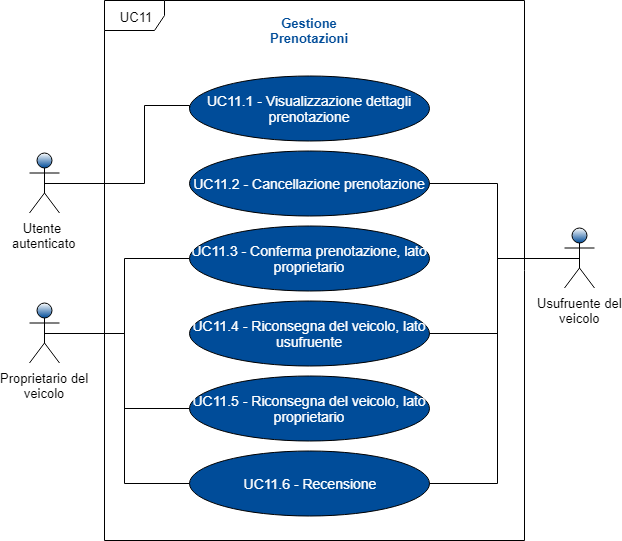
\includegraphics[width=10cm]{res/images/UC11Prenotazione.png}
	\centering
	\caption{UC11 - Gestione prenotazione}
\end{figure}
\begin{itemize}
	\item \textbf{Attori Primari}: utente autenticato;
	\item \textbf{Descrizione}: agli utenti autenticati è resa disponibile una maschera che presenta la lista di tutte le sue prenotazioni ancora attive, dalla quale l'utente può scegliere di effettuare operazioni di gestione su ognuna di esse;
	per ogni prenotazione presente nella lista saranno visualizzati dei dettagli riassuntivi, che sono:
	\begin{itemize}
		\item nome del proprietario del veicolo o dell'usufruente;
		\item data;
		\item fascia oraria;
		\item marca del veicolo prenotato;
		\item modello del veicolo prenotato;
		\item anno d'immatricolazione del veicolo prenotato.
	\end{itemize}
	\item \textbf{Scenario principale}: l'utente effettua operazioni di gestione di una prenotazione. Esse comprendono:
	\begin{itemize}
		\item visualizzazione dettagli prenotazione [UC11.1];
		\item cancellazione prenotazione [UC11.2].
	\end{itemize}
	\item \textbf{Scenario secondario}: il proprietario di un veicolo, inoltre potrà confermare le prenotazioni ricevute [UC11.3];
	\item \textbf{Precondizione}: il sistema carica correttamente la lista delle prenotazioni effettuate attualmente attive;
	\item \textbf{Post-condizione}: l'utente ha visualizzato le sue prenotazioni correnti ed è riuscito ad effettuare eventuali modifiche.
\end{itemize} 
 \subsubsection{UC11.1 - Visualizzazione dettagli prenotazione}
\begin{itemize}
	\item \textbf{Attori Primari}: utente autenticato;
	\item \textbf{Descrizione}: l'utente visualizza i dettagli della prenotazione scelta dalla maschera di presentazione delle prenotazioni, ciò gli permette di visualizzare:
	\begin{itemize}
		\item nome del proprietario del veicolo o dell'usufruente;
		\item la data;
		\item la fascia oraria;
		\item il veicolo prenotato;
	\end{itemize}
	Inoltre se presenti, verranno visualizzati anche:
	\begin{itemize}		
		\item il luogo d'incontro;
		\item l'orario d'incontro;
	\end{itemize}
	\item \textbf{Scenario principale}: L'utente visualizza i dettagli della prenotazione.	
	\item \textbf{Precondizione}: l'utente ha scelto una prenotazione;
	\item \textbf{Post-condizione}: l'utente ha visualizzato correttamente i dettagli della prenotazione.
\end{itemize}
\begin{comment}

\end{comment}
\subsubsection{UC11.2 - Cancellazione prenotazione}
\begin{itemize}
	\item \textbf{Attori Primari}: utente autenticato;
	\item \textbf{Descrizione}: l'utente cancella la prenotazione selezionata;
	\item \textbf{Scenario principale}: l'utente si trova all'interno della pagina di visualizzazione dei dettagli della prenotazione precedentemente selezionata. Attraverso l'apposito pulsante l'utente chiederà la cancellazione della prenotazione;
	\item \textbf{Precondizione}: l'utente ha premuto il pulsante per la cancellazione delle prenotazione precedentemente selezionata;
	\item \textbf{Post-condizione}: l'utente ha annullato correttamente la prenotazione selezionata.
\end{itemize}

\subsubsection{UC11.3 - Conferma prenotazioni, lato proprietario}
\begin{itemize}
	\item \textbf{Attori Primari}: proprietario del veicolo;
	\item \textbf{Descrizione}: il proprietario del veicolo conferma o annulla la richiesta di prenotazione ricevuta;
	\item \textbf{Scenario principale}: l'utente si trova all'interno della pagina di visualizzazione dei dettagli della richiesta di prenotazione appena ricevuta. Attraverso gli appositi campi l'utente potrà specificare:
	\begin{itemize}
		\item luogo d'incontro [UC11.3.1];
		\item orario d'incontro [UC11.3.2].
	\end{itemize} 
	\item \textbf{Precondizione}: l'utente visualizza correttamente la prenotazione che intende confermare o annullare;
	\item \textbf{Post-condizione}: l'utente ha confermato o annullato correttamente la richiesta di prenotazione ricevuta.
\end{itemize}
\begin{figure}[h]
	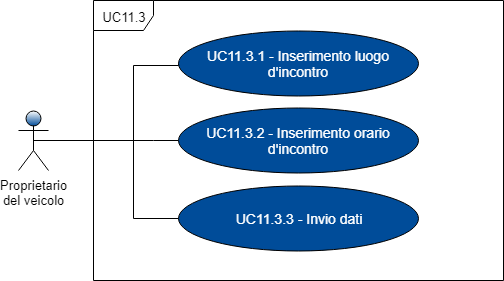
\includegraphics[width=10cm]{res/images/UC11-3Conferma.png}
	\centering
	\caption{UC11.3 - Conferma prenotazioni, lato proprietario}
\end{figure}

\subsubsection{UC11.3.1 - Inserimento luogo d'incontro}
\begin{itemize}
	\item \textbf{Attori Primari}: proprietario del veicolo;
	\item \textbf{Descrizione}: al fine di portare a termine il processo di conferma della prenotazione, l'utente deve inserire il luogo d'incontro, campo ritenuto obbligatorio;
	\item \textbf{Scenario principale}: l'utente compila il campo relativo al luogo d'incontro;	
	\item \textbf{Precondizione}: l'applicazione ha reso disponibile il campo per l'inserimento del luogo d'incontro;
	\item \textbf{Postcondizione}: l'utente ha compilato il campo con il luogo d'incontro.	
\end{itemize}

\subsubsection{UC11.3.2 - Inserimento orario d'incontro}
\begin{itemize}
	\item \textbf{Attori Primari}: proprietario del veicolo;
	\item \textbf{Descrizione}: al fine di portare a termine il processo di conferma della prenotazione, l'utente deve inserire l'orario d'incontro, campo ritenuto obbligatorio;
	\item \textbf{Scenario principale}: l'utente compila il campo relativo all'orario d'incontro;	
	\item \textbf{Precondizione}: l'applicazione ha reso disponibile il campo per l'inserimento dell'orario d'incontro;
	\item \textbf{Postcondizione}: l'utente ha compilato il campo con l'orario d'incontro.	
\end{itemize}

\subsubsection{UC11.3.3 - Invio dati}
\begin{itemize}
	\item \textbf{Attori Primari}: proprietario del veicolo;
	\item \textbf{Descrizione}: l'utente preme il pulsante per la conferma e l'invio dei dati;
	\item \textbf{Scenario principale}: l'utente preme il pulsante di verifica ed invio dei dati;	
	\item \textbf{Precondizione}: l'utente ha compilato i dati necessari per la conferma della prenotazione e preme il pulsante per l'invio dei dati;
	\item \textbf{Postcondizione}: la prenotazione viene confermata.
\end{itemize}

\subsubsection{UC11.4 - Riconsegna del veicolo, lato usufruente}
\begin{itemize}
	\item \textbf{Attori Primari}: usufruente del veicolo;
	\item \textbf{Descrizione}: l'utente riconsegna il veicolo e chiude la prenotazione;
	\item \textbf{Scenario principale}: l'utente si trova all'interno della pagina di visualizzazione dei dettagli della prenotazione precedentemente selezionata. Dopo aver riconsegnato il veicolo e le chiavi, attraverso l'apposito pulsante l'utente chiederà la chiusura della prenotazione (la prenotazione verrà definitivamente chiusa quando anche il proprietario del veicolo confermerà la riconsegna delle chiavi e del mezzo [UC11.5]). Comparirà un pop-up che permetterà di lasciare una recensione all'altro utente [UC11.6];
	\item \textbf{Inclusioni}: 
	\begin{itemize}
		\item recensione utente [UC11.6].
	\end{itemize}
	\item \textbf{Precondizione}: l'utente visualizza correttamente la prenotazione che intende concludere;
	\item \textbf{Post-condizione}: l'utente ha richiesto correttamente la chiusura della prenotazione selezionata.
	
\end{itemize}

\subsubsection{UC11.5 - Riconsegna del veicolo, lato proprietario}
\begin{itemize}
	\item \textbf{Attori Primari}: proprietario del veicolo;
	\item \textbf{Descrizione}: il proprietario del veicolo conferma la riconsegna del mezzo e delle chiavi;
	\item \textbf{Scenario principale}: l'utente si trova all'interno della pagina di visualizzazione dei dettagli della prenotazione precedentemente selezionata. Alla riconsegna del veicolo e delle chiavi, attraverso l'apposito pulsante l'utente confermerà la chiusura della prenotazione in modo definitivo. Comparirà un pop-up che permetterà di lasciare una recensione all'altro utente [UC11.6];
	\item \textbf{Inclusioni}: 
	\begin{itemize}
		\item recensione utente [UC11.6].
	\end{itemize}
	\item \textbf{Precondizione}: l'utente visualizza correttamente la prenotazione che intende concludere;
	\item \textbf{Post-condizione}: l'utente ha concluso correttamente la prenotazione selezionata.
\end{itemize}

\subsubsection{UC11.6 - Recensione}
\begin{itemize}
	\item \textbf{Attori Primari}: utente autenticato;
	\item \textbf{Descrizione}: l'utente recensisce l'altro utente coinvolto nella prenotazione;
	\item \textbf{Scenario principale}: l'utente visualizza il pop-up per inserire la recensione che consiste in una valutazione da una a cinque stelle;
	\item \textbf{Precondizione}: l'utente visualizza correttamente il pop-up;
	\item \textbf{Post-condizione}: l'utente ha inserito correttamente la recensione.
\end{itemize}

